\documentclass[]{../template/Report}%方括号内写yuxi即生成预习报告
\settemplatedir{../template/}%设置模板路径

\exname{金属材料杨氏模量的测定} %实验名称
\extable{11} %实验桌号
\instructor{王宙洋} %指导教师
\class{信工2401} %班级
\name{姚舜瑜} %姓名
\stuid{3240100532} %学号

\nyear{2025} %年
\nmonth{11} %月
\nday{18} %日
\nweekday{二} %星期几，e.g. \nweekday{三}
\daypart{上午}%上午/下午

\redate{} %如有实验补做，补做日期
\resitu{} %情况说明：

\begin{document}
\maketitle%输出封面

\section{预习报告（10分）}
\subsection{实验综述}
\subsubsection{实验目的}
通过光杠杆法测定金属丝的杨氏模量 $E$；理解并掌握光杠杆放大量测小形变的思想与逐差法的数据处理。

\subsubsection{实验原理}
杨氏模量用于量化材料在弹性形变范围内的刚度。在弹性限度内，金属材料遵循胡克定律：应力（$F/S$）与应变（$\Delta L/L$）成正比，其比例系数定义为杨氏模量
\[E = \frac{F\,L}{S\,\Delta L}.\]
其中，应力是指单位面积上所受到的垂直力，也就是$F/S$；应变是指材料长度的相对变化，也就是$\Delta L/L$。
本实验采用光杠杆法放大钢丝的微小伸长以便读数。实验装置见\cref{shiyanzhuangzhi}。

\begin{figure}[H]
    \centering
    
\includegraphics[width=0.75\textwidth]{shiyanzhuangzhi.png}
    \caption{金属材料杨氏模量测定的实验装置}
    \label{shiyanzhuangzhi}
\end{figure}

光杠杆镜是一块三足平面镜（见\cref{guanggangganjing}），三足尖 $O_1,O_2,O_3$ 构成等腰三角形，顶点 $O_3$ 到底边的距离为 $b$。标尺经平面镜反射后在望远镜中成像，初读数记为 $s_0$。

\begin{figure}[H]
    \centering
    \begin{minipage}{0.45\textwidth}
        \centering
    
\includegraphics[height=4cm,keepaspectratio]{guanggangganjing.png}
    \caption{光杠杆镜}
    \label{guanggangganjing}
    \end{minipage}
    \begin{minipage}{0.45\textwidth}
        \centering
        
\includegraphics[height=4cm,keepaspectratio]{guanglutu.png}
        \caption{光杠杆光路示意图}
        \label{guanglutu}
    \end{minipage}    
\end{figure}

当保持 $O_1,O_2$ 在同一平台上、$O_3$ 因钢丝伸长下降 $\Delta L$ 时，平面镜转过角度 $\theta$，望远镜读数由 $s_0$ 变为 $s_1$（光路如\cref{guanglutu}）。几何关系为
\[\frac{\Delta s}{D}=\tan 2\theta\approx 2\theta,\qquad \frac{\Delta L}{b}=\tan\theta\approx\theta,\]
由此得到光杠杆的线位移放大关系
\[\Delta s = \frac{2D}{b}\,\Delta L,\]
其中 $D$ 为标尺与镜面间距离，$\tfrac{2D}{b}$ 为光杠杆常数（通常 $\gg 1$）。



钢丝截面积 $S=\tfrac{\pi d^2}{4}$（$d$ 为直径）。代入上式并以砝码质量 $m$ 产生拉力 $F=mg$，可得杨氏模量的计算式
\[\bar{E}=\frac{8DmgL}{\pi d^2 b\,\Delta s}.\]

\subsubsection{实验步骤}
\begin{enumerate}
    \item 预备实验：用螺旋测微计（多部位）测钢丝直径 $d$；用米尺测原长 $L$；用卷尺测标尺到镜面的距离 $D$；将光杠杆三足在白纸上压痕后，用直尺连两前脚、以游标卡尺测后脚到该连线的垂直距离 $b$。各量多次测量取平均。
    \item 仪器调校：支架调至铅直、钢丝拉直且夹具无接触；反射镜面竖直；望远镜对焦、与光路共轴并消除视差。
    \item 载荷与读数：逐个增加砝码至最大后再逐个减小，记录每一步的砝码质量与标尺读数（共 8 组不同质量）。对相应的上、下行读数 $s_i$ 与 $s_i'$ 取平均，并用逐差法求
    \[\Delta s_i=\frac{s_{i+4}-s_i}{4},\quad i=0,1,2,3.\]
    \item 数据处理：计算各组数据的杨氏模量 $E_i$，并求其平均值 $\bar{E}$ ，并进行不确定度分析。
\end{enumerate}

\subsection{实验重点}
\begin{enumerate}
\item 掌握杨氏模量的物理意义及拉伸法测量原理
\item 理解光杠杆放大原理，熟练掌握光路调节技术
\item 学会用逐差法处理数据，掌握不确定度的计算方法
\end{enumerate}

\subsection{实验难点}
本实验的主要操作难点体现在以下几个方面：

\begin{enumerate}
\item \textbf{仪器初调}：调水平仪使底座水平、立柱铅直，金属丝竖直且不与孔壁接触，上下夹具夹紧。
\item \textbf{光路调节}：调节反射镜使其竖直，调望远镜使光轴与镜面共轴，并消除视差，使标尺像与叉丝清晰重合。
\item \textbf{异常处理}：标尺像丢失时，按顺序检查并微调光路；读数异常时，检查夹头是否松动、装置是否倾斜，注意避免超过弹性限度。
\item \textbf{数据处理}：用逐差法处理读数，计算杨氏模量并进行不确定度分析，确保结果的准确性和可靠性。
\end{enumerate}


\begin{fullreportonly}
\section{原始数据（20分）}
\begin{figure}[H]
    \centering
    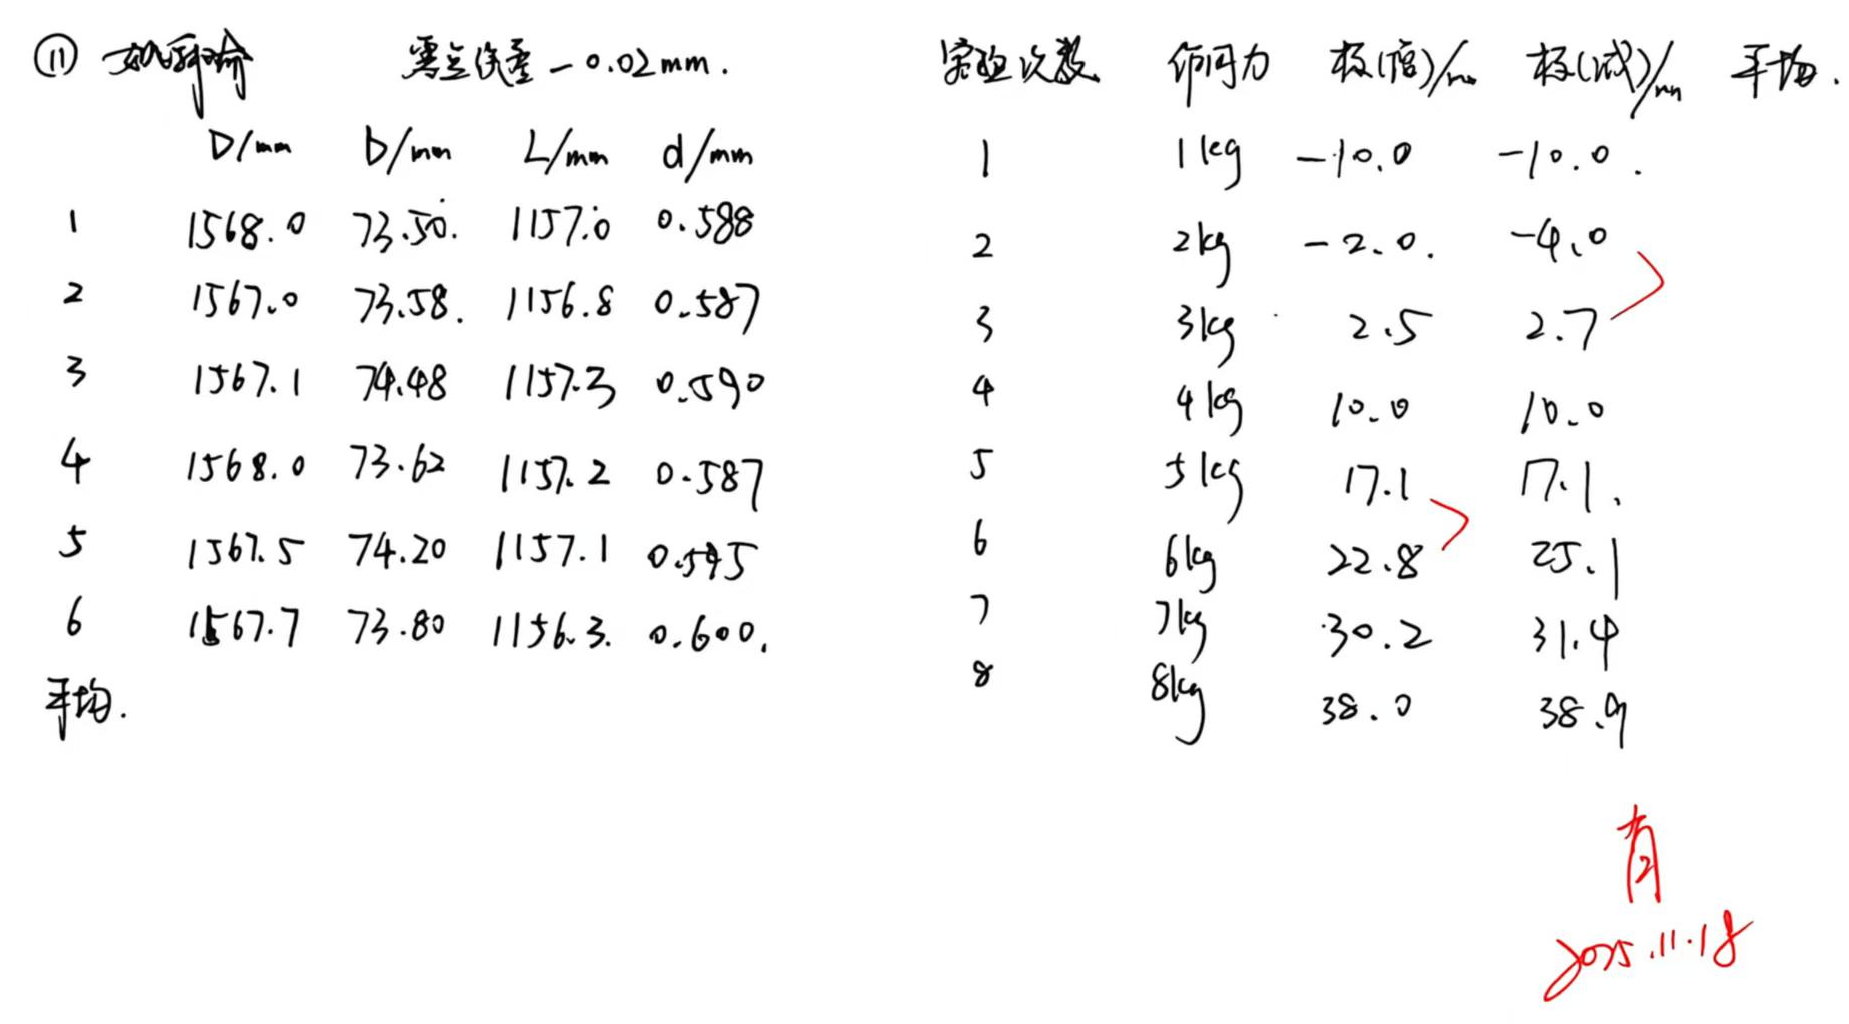
\includegraphics[width=0.6\textwidth]{figures/Y数据.png}
    \caption{实验原始数据记录表}
    \label{shuju}
\end{figure}

\section{结果与分析（60分）}
\subsection{数据处理与结果（30分）}
\subsubsection{装置几何参数预测量}

\begin{table}[H]
    \centering
    \caption{装置几何参数测量数据}
    \label{tab:geom_params}
    \small
    \begin{tabular}{|c|c|c|c|c|}
        \hline
        序号 & $D$/mm & $b$/mm & $L$/mm & $d$/mm \\
        \hline
        1 & 1568.0 & 73.50 & 1157.0 & 0.588 \\
        2 & 1567.0 & 73.58 & 1156.8 & 0.587 \\
        3 & 1567.1 & 74.48 & 1157.3 & 0.590 \\
        4 & 1568.0 & 73.62 & 1157.2 & 0.587 \\
        5 & 1567.5 & 74.20 & 1157.1 & 0.595 \\
        6 & 1567.7 & 73.80 & 1156.3 & 0.600 \\
        \hline
    平均& 1567.55 & 73.86 & 1156.95 & 0.591 \\
        \hline
    \end{tabular}
\end{table}
\subsubsection{计算与结果}
取表~\ref{tab:geom_params} 平均值：\(D=1567.55\,\mathrm{mm},\ b=73.86\,\mathrm{mm},\ L=1156.95\,\mathrm{mm},\ d=0.591\,\mathrm{mm}\)。令杭州市重力加速度 \(g=9.7936\,\mathrm{m/s^2}\)。对表~\ref{tab:load_readings} 读数取平均，得
\[s=\{-10.0,\,-3.0,\,2.6,\,10.0,\,17.1,\,23.95,\,30.8,\,38.45\}\,\mathrm{mm} .\]

(1) 逐差法：按 \(\Delta s_i=\frac{s_{i+4}-s_i}{4}\,(i=1,2,3,4)\) 得
\[\Delta s=\{6.775,\,6.7375,\,7.0500,\,7.1125\}\,\mathrm{mm/\,kg},\quad \overline{\Delta s}=6.91875\,\mathrm{mm/\,kg}.\]
代入
\[\bar{E}=\frac{8DmgL}{\pi d^2 b\,\Delta s}\]
并令 \(m=1\,\mathrm{kg}\)（逐差法得到的是每千克的平均读数增量），统一至 SI 单位，计算得
\[\boxed{\bar{E}_{\text{逐差}}\approx 2.532\times10^{11}\,\mathrm{Pa}\ (=253.2\,\mathrm{GPa})}.\]

(2) 线性拟合法：对 \(s\) 与 \(m\) 最小二乘拟合 \(s=k\,m+c\) 得斜率 \(k\approx 6.89643\,\mathrm{mm/\,kg}\)。由
\[\Delta s=\frac{2D}{b}\,\frac{m g L}{S E}\ \Rightarrow\ E=\frac{2D g L}{b S k},\qquad S=\frac{\pi d^2}{4},\]
代入同一组几何与物理量得
\[\boxed{\bar{E}_{\text{拟合}}\approx 2.541\times10^{11}\,\mathrm{Pa}\ (=254.1\,\mathrm{GPa})}.\]
两种方法结果一致，差异小于 1\%。

\begin{figure}[H]
    \centering
    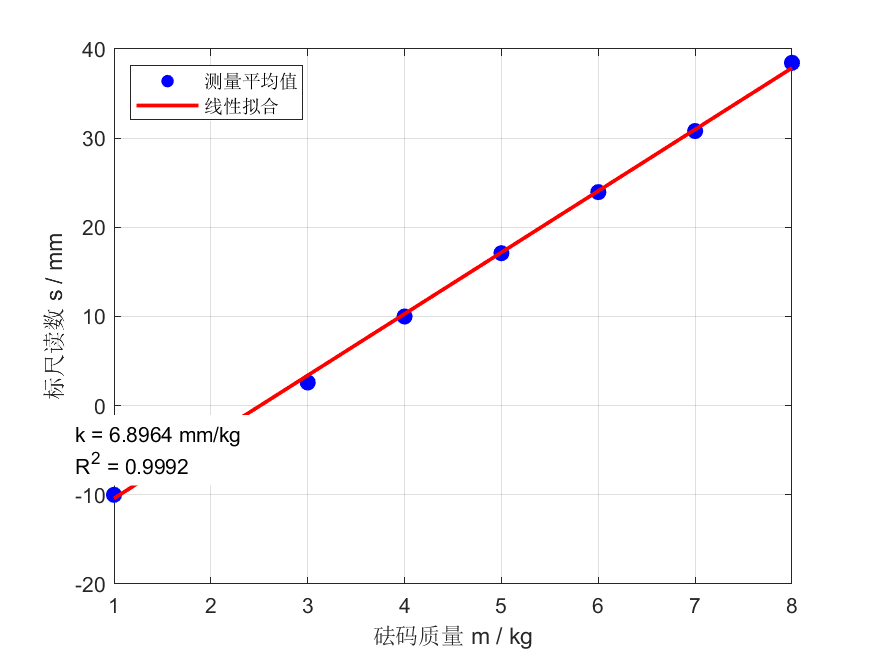
\includegraphics[width=0.72\textwidth]{figures/Y_fit.png}
    \caption{$s$–$m$ 散点与线性拟合示意（脚本运行后自动生成）；图注含斜率、截距、$R^2$}
    \label{fig:Y_fit}
\end{figure}

\subsubsection{杨氏模量计算数据测量}
\begin{table}[H]
    \centering
    \caption{杨氏模量计算数据测量}
    \label{tab:load_readings}
    \small
    \begin{tabular}{|c|c|c|c|c|}
        \hline
        实验序号 & 砝码质量/kg & 增砝码时读数/mm & 减砝码时读数/mm & 平均 \\
        \hline
        1 & 1 & -10.0 & -10.0 & -10.0 \\
        2 & 2 & -2.0 & -4.0 & -3.0 \\
        3 & 3 & 2.5 & 2.7 & 2.6 \\
        4 & 4 & 10.0 & 10.0 & 10.0 \\
        5 & 5 & 17.1 & 17.1 & 17.1 \\
        6 & 6 & 22.8 & 25.1 & 23.95 \\
        7 & 7 & 30.2 & 31.4 & 30.8 \\
        8 & 8 & 38.0 & 38.9 & 38.45 \\
        \hline
    \end{tabular}
\end{table}
\subsection{误差分析（20分）}
（运用测量误差、相对误差或不确定度等分析实验结果，写出完整的结果表达式，并分析误差原因。）

\subsection{实验探讨（10分）}
（对实验内容、现象和过程的小结，不超过100字。）

\section{思考题（10分）}
（解答教材或讲义或老师布置的思考题，请先写题干，再作答。）
\end{fullreportonly}
\insertnotes
\end{document}